\section{Mô hình Nền tảng cho các Tác vụ Thị giác}
\label{sec:foundation_models_vision_tasks}

\subsection{Giới thiệu: Sự trỗi dậy của các "Bộ não" Thị giác Đa năng}
\label{subsec:foundation_models_intro}
Trong suốt các phần trước của chương này, chúng ta đã khám phá các kiến trúc được thiết kế chuyên biệt để giải quyết các tác vụ cụ thể: YOLO cho phát hiện vật thể, U-Net và Mask R-CNN cho phân đoạn, HRNet cho ước tính tư thế. Mỗi mô hình là một "chuyên gia" trong lĩnh vực của nó, được huấn luyện và tối ưu hóa cho một mục tiêu duy nhất.

Tuy nhiên, từ khoảng năm 2023 trở đi, một làn sóng mới, kế thừa triết lý từ các mô hình ngôn ngữ lớn (LLMs) như GPT, đã bắt đầu định hình lại toàn bộ lĩnh vực. Đó là kỷ nguyên của các \textbf{Mô hình Nền tảng (Foundation Models)} cho thị giác.

\begin{mdframed}[style=infobox]
	\textbf{Định nghĩa Mô hình Nền tảng Thị giác}
	
	Một mô hình nền tảng thị giác là một mô hình quy mô lớn, được huấn luyện trước (pre-trained) trên một lượng dữ liệu khổng lồ và đa dạng (thường là đa phương thức). Thay vì học để giải quyết một tác vụ duy nhất, nó học các \textbf{biểu diễn tổng quát (general-purpose representations)} và các khả năng cốt lõi (core capabilities). Mô hình này sau đó có thể được thích ứng (adapted) một cách hiệu quả để giải quyết hàng loạt các tác vụ xuôi dòng (downstream tasks) khác nhau, thường chỉ với ít hoặc không cần dữ liệu gán nhãn bổ sung.
\end{mdframed}

Sự chuyển dịch này đánh dấu một bước ngoặt: từ việc xây dựng nhiều "công cụ" chuyên biệt sang việc xây dựng một "bộ não" thị giác đa năng. Thay vì hỏi "Kiến trúc nào tốt nhất cho việc phát hiện?", chúng ta bắt đầu hỏi "Làm thế nào để 'ra lệnh' cho một mô hình nền tảng thực hiện việc phát hiện?". Phần này sẽ khám phá ba trong số những mô hình nền tảng tiên phong đã định nghĩa lại các tác vụ thị giác cốt lõi.

\subsection{Grounding DINO (2023): Phát hiện Mọi thứ bằng Ngôn ngữ}
\label{subsec:grounding_dino}

\textbf{Grounding DINO} \cite{Liu2023_GroundingDINO} là một mô hình mở ra khả năng \textbf{phát hiện vật thể theo ngôn ngữ}, chuyển từ "closed-set detection" sang \textbf{open-vocabulary detection}.

\textbf{Vấn đề của các mô hình truyền thống:}  
Các detector như YOLO, Faster R-CNN chỉ nhận diện các lớp đã thấy trong huấn luyện. Việc mở rộng sang các lớp mới đòi hỏi dữ liệu và huấn luyện lại.

\textbf{Ý tưởng cốt lõi:}  
Grounding DINO kết hợp hai yếu tố:
\begin{enumerate}
	\item \textbf{Phát hiện End-to-End:} Sử dụng kiến trúc Transformer encoder-decoder của DINO để dự đoán trực tiếp các bounding box.
	\item \textbf{Hiểu ngôn ngữ:} Các object query được \textbf{grounded} vào embedding văn bản từ prompt, thay vì học query mù mờ.
\end{enumerate}

---

\textbf{Kiến trúc và pipeline:}

\begin{enumerate}
	\item \textbf{Input:} Ảnh $I$ và prompt văn bản $T$.
	\item \textbf{Feature Extraction:}
	\[
	F_I = \text{ImageEncoder}(I), \quad F_T = \text{TextEncoder}(T)
	\]
	với $F_I \in \mathbb{R}^{H \times W \times C}$ và $F_T \in \mathbb{R}^{L \times D}$.
	\item \textbf{Cross-Modality Attention:} Decoder thực hiện attention giữa text queries $q_t \in F_T$ và các patch embedding $p_i \in F_I$:
	\[
	\text{Attention}(q_t, F_I) = \text{Softmax}\Big(\frac{q_t K^T}{\sqrt{d}}\Big) V
	\]
	với $K, V$ là key và value từ feature map hình ảnh. Kết quả là mỗi query học được trọng số cho các vùng ảnh liên quan.
	\item \textbf{Prediction Head:} Mỗi query đưa qua FFN để dự đoán bounding box $(x, y, w, h)$ và score liên quan đến cụm từ trong prompt:
	\[
	(x, y, w, h, s) = \text{FFN}(\text{Attention}(q_t, F_I))
	\]
\end{enumerate}

\textbf{Hàm mất mát:}  
Grounding DINO huấn luyện bằng cách kết hợp:
\begin{itemize}
	\item \textbf{Hungarian bipartite matching:} Gán mỗi prediction với ground-truth phrase để tối ưu một-một.
	\item \textbf{Box regression loss:} $\mathcal{L}_{box} = \text{L1}(b_\text{pred}, b_\text{gt}) + \text{GIoU}(b_\text{pred}, b_\text{gt})$
	\item \textbf{Score matching loss:} $\mathcal{L}_{cls} = - \sum_i y_i \log s_i$
\end{itemize}

\textbf{Trực giác:}  
Mỗi query văn bản học cách "tìm kiếm" trong feature map hình ảnh những vùng liên quan đến ý nghĩa ngôn ngữ. Attention hoạt động như một bản đồ trọng số, hướng decoder tập trung vào các đối tượng đúng.

\begin{center}
	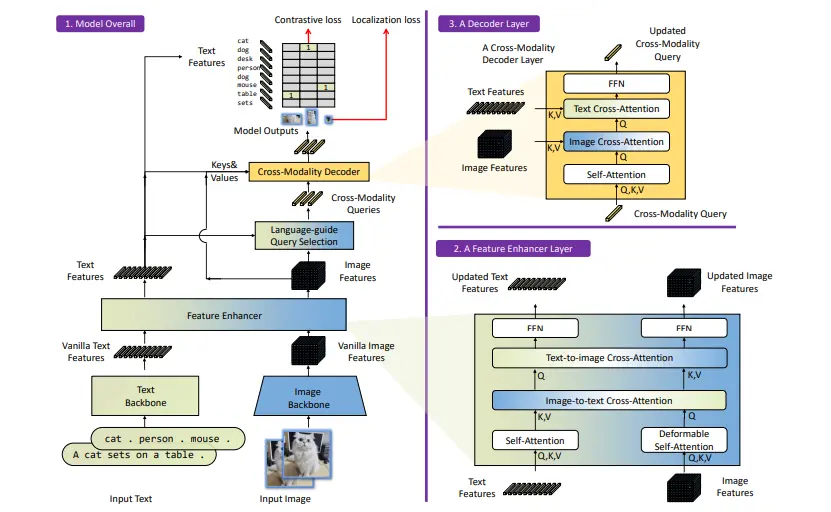
\includegraphics[width=1.0\textwidth]{images/grounding_dino_architecture.png}
	\captionof{figure}{Sơ đồ kiến trúc Grounding DINO: ảnh và văn bản được mã hóa riêng, decoder thực hiện cross-modality attention, dự đoán bounding box và score cho từng cụm từ.}
	\label{fig:grounding_dino_architecture}
\end{center}

\textbf{Tầm ảnh hưởng:}  
Grounding DINO cho phép phát hiện \textbf{mọi vật thể có thể mô tả bằng ngôn ngữ}, là nền tảng cho các hệ thống như \textbf{Grounded-SAM}, mở ra khả năng \textbf{programmable object detection}.

\subsection{Florence-2 (Microsoft, 2023): Xương sống Thị giác Toàn năng}
\label{subsec:florence_2}

\textbf{Florence-2} \cite{Zhang2023_Florence2} là nỗ lực xây dựng một \textbf{universal visual encoder}, có thể phục vụ cho nhiều tác vụ thị giác khác nhau mà không cần huấn luyện riêng lẻ.

\textbf{Triết lý cốt lõi:} 
Thay vì huấn luyện riêng cho từng tác vụ (CLIP cho contrastive, MAE cho tự động hóa), Florence-2 học một không gian biểu diễn thống nhất, có khả năng điều chỉnh hành vi thông qua \textbf{task prompts}.

---

\textbf{Kiến trúc:}  
Florence-2 sử dụng một \textbf{Transformer encoder-decoder}:
\[
F_I = \text{ImageEncoder}(I), \quad F_T = \text{TaskPromptEncoder}(p_\text{task})
\]
với $I$ là ảnh đầu vào, $p_\text{task}$ là prompt của tác vụ (ví dụ: `<OD>` cho object detection, `<CAPTION>` cho captioning).

Decoder thực hiện cross-attention giữa $F_I$ và embedding của prompt $F_T$:
\[
\text{Attention}(F_T, F_I) = \text{Softmax}\Big(\frac{F_T K_I^T}{\sqrt{d}}\Big) V_I
\]
trong đó $K_I, V_I$ là key và value từ image encoder, $d$ là chiều embedding.

---

\textbf{Huấn luyện đa nhiệm:}  
Florence-2 được huấn luyện đồng thời trên nhiều tác vụ:
\begin{enumerate}
	\item \textbf{Image-Text Contrastive:}  
	Giúp ánh xạ ảnh và văn bản vào cùng không gian embedding. Hàm mất mát tiêu chuẩn:
	\[
	\mathcal{L}_\text{ITC} = - \log \frac{\exp(\text{sim}(F_I, F_T)/\tau)}{\sum_j \exp(\text{sim}(F_I, F_{T_j})/\tau)}
	\]
	với $\text{sim}(\cdot)$ là cosine similarity, $\tau$ là temperature.
	
	\item \textbf{Captioning:}  
	Sử dụng cross-entropy loss dự đoán token chuỗi văn bản:
	\[
	\mathcal{L}_\text{CAP} = - \sum_{t=1}^{L} \log P(y_t | y_{<t}, F_I, F_T)
	\]
	
	\item \textbf{Object Detection:}  
	Sử dụng bipartite matching loss, kết hợp L1 và GIoU:
	\[
	\mathcal{L}_\text{OD} = \lambda_1 \text{L1}(b_\text{pred}, b_\text{gt}) + \lambda_2 \text{GIoU}(b_\text{pred}, b_\text{gt})
	\]
	
	\item \textbf{Grounding:}  
	Kết hợp object queries với các khu vực ảnh tương ứng của chú thích:
	\[
	\mathcal{L}_\text{GRD} = - \sum_i y_i \log s_i
	\]
\end{enumerate}

Tổng loss huấn luyện là tổng có trọng số của các thành phần:
\[
\mathcal{L}_\text{total} = \alpha \mathcal{L}_\text{ITC} + \beta \mathcal{L}_\text{CAP} + \gamma \mathcal{L}_\text{OD} + \delta \mathcal{L}_\text{GRD}
\]

---

\textbf{Trực giác:}  
\begin{itemize}
	\item Các task prompt hướng decoder tập trung vào phần embedding cần thiết cho từng tác vụ.
	\item Cross-attention cho phép mô hình vừa hiểu ngữ nghĩa toàn cục của ảnh, vừa kết hợp với thông tin đặc thù của tác vụ.
	\item Mạng học được một \textbf{không gian biểu diễn chung} mà mọi tác vụ thị giác có thể tận dụng.
\end{itemize}

\textbf{Tầm ảnh hưởng:}  
Florence-2 là xương sống cho các hệ thống thị giác toàn năng:
\begin{itemize}
	\item Thực hiện zero-shot/few-shot trên phân loại, phát hiện, phân đoạn, captioning, VQA.
	\item Thể hiện sức mạnh của biểu diễn thống nhất, cho phép tích hợp nhanh các mô hình nền tảng khác.
\end{itemize}

\subsection{Kosmos-2 (Microsoft, 2023): Mô hình Ngôn ngữ Lớn Đa phương thức}
\label{subsec:kosmos_2}

\textbf{Kosmos-2} \cite{Peng2023_Kosmos2} là một \textbf{Large Multimodal Model (LMM)} thực thụ, kết hợp thị giác và ngôn ngữ trong một không gian biểu diễn thống nhất.

\textbf{Triết lý: Grounded Multimodal Language Modeling}  
Kosmos-2 coi các vùng ảnh và đối tượng như "token đặc biệt", cho phép mô hình vừa hiểu, vừa mô tả, vừa gắn kết (ground) thông tin trong ảnh.

---

\textbf{Kiến trúc:}  
\begin{itemize}
	\item \textbf{Image Encoder:} Một Vision Transformer hoặc Swin Transformer trích xuất embedding $F_I$ từ ảnh.
	\item \textbf{Text Encoder / Decoder:} Một LLM (ví dụ GPT-like) học embedding $F_T$ từ văn bản, và có khả năng sinh chuỗi token.
	\item \textbf{Cross-Modality Grounding:} Sử dụng cross-attention giữa $F_T$ và $F_I$:
	\[
	\text{Attention}(F_T, F_I) = \text{Softmax}\Big(\frac{F_T K_I^T}{\sqrt{d}}\Big)V_I
	\]
	để liên kết các token ngôn ngữ với các vùng ảnh tương ứng.
\end{itemize}

---

\textbf{Huấn luyện:} Kosmos-2 học đồng thời nhiều tác vụ:
\begin{enumerate}
	\item \textbf{Text Generation / Captioning:}
	\[
	\mathcal{L}_\text{CAP} = -\sum_{t=1}^L \log P(y_t | y_{<t}, F_I)
	\]
	giúp mô hình tạo mô tả ảnh.
	
	\item \textbf{Grounding / Region-Text Alignment:} 
	\[
	\mathcal{L}_\text{GRD} = - \sum_i y_i \log s_i
	\]
	trong đó $s_i$ là xác suất token văn bản $i$ được gắn với đúng bounding box.
	
	\item \textbf{Contrastive Alignment (Ảnh - Ngôn ngữ):}  
	Tương tự CLIP, để ánh xạ ảnh và văn bản vào cùng embedding space:
	\[
	\mathcal{L}_\text{ITC} = - \log \frac{\exp(\text{sim}(F_I, F_T)/\tau)}{\sum_j \exp(\text{sim}(F_I, F_{T_j})/\tau)}
	\]
\end{enumerate}

Tổng loss huấn luyện có thể viết như:
\[
\mathcal{L}_\text{total} = \alpha \mathcal{L}_\text{CAP} + \beta \mathcal{L}_\text{GRD} + \gamma \mathcal{L}_\text{ITC}
\]

---

\textbf{Trực giác:}  
\begin{itemize}
	\item Cross-attention cho phép mô hình "tìm kiếm" vùng ảnh liên quan đến token văn bản.
	\item Token ảnh và token văn bản được học trong cùng không gian biểu diễn, giúp mô hình thực hiện **zero-shot grounding**.
	\item Task prompts hoặc instruction text hướng Kosmos-2 thực hiện các nhiệm vụ khác nhau (mô tả, hỏi đáp, phân đoạn, hoặc chỉ bounding box cụ thể).
\end{itemize}

\textbf{Tầm ảnh hưởng:}  
Kosmos-2 và các LMM kế thừa (như LLaVA, GPT-4o, Gemini) là bước tiến hướng tới AI "có thị giác và ngôn ngữ tích hợp", mở ra:
\begin{itemize}
	\item Tương tác với AI qua ảnh và văn bản.
	\item Hệ thống robot nhận diện và thao tác dựa trên mô tả ngôn ngữ.
	\item Hệ thống truy vấn kiến thức hình ảnh-text zero-shot.
\end{itemize}

\subsection{Kết luận: Một Mô hình cho Mọi Tác vụ}
\label{subsec:foundation_models_conclusion}
Sự trỗi dậy của các mô hình nền tảng như Grounding DINO, Florence-2, và Kosmos-2 đang làm thay đổi căn bản kiến trúc và quy trình làm việc trong thị giác máy tính.
\begin{itemize}
	\item \textbf{Sự Hội tụ của các Tác vụ:} Ranh giới giữa phân loại, phát hiện, và phân đoạn đang dần bị xóa nhòa. Một mô hình duy nhất, có khả năng lý luận đa phương thức, có thể được "prompt" để giải quyết tất cả các tác vụ này.
	\item \textbf{Từ Chuyên gia đến Đa năng:} Thay vì xây dựng hàng trăm "chuyên gia" hẹp, ngành công nghiệp đang hướng tới việc xây dựng và tinh chỉnh các mô hình "đa năng" (generalist) khổng lồ.
	\item \textbf{Biểu diễn là Giao diện (Representation as an API):} Các mô hình nền tảng cung cấp các biểu diễn thị giác-ngôn ngữ như một dịch vụ. Các ứng dụng xuôi dòng có thể xây dựng dựa trên các biểu diễn này mà không cần phải huấn luyện lại các mô hình khổng lồ từ đầu.
\end{itemize}
Tương lai của thị giác máy tính đang tiến nhanh tới một viễn cảnh của \textbf{AI Tổng quát}, nơi nhận thức (perception), lý luận (reasoning), và hành động (action) được hợp nhất trong các mô hình thống nhất, có khả năng hiểu và tương tác với thế giới đa phương thức của chúng ta một cách liền mạch.

\section*{Tài liệu tham khảo}
\begin{itemize}
	\item[1] Liu, S., Li, Z., Li, H., Zhang, J., Su, H., Zhu, J., ... \& Wang, J. (2023). Grounding dino: Marrying dino with grounded pre-training for open-set object detection. \textit{arXiv preprint arXiv:2303.05499}. (Paper gốc giới thiệu Grounding DINO).
	\item[2] Zhang, P., et al. (2023). Florence-2: A novel vision foundation model for universal image-text representation. \textit{Microsoft AI Blog \& Technical Report}. (Báo cáo kỹ thuật giới thiệu Florence-2).
	\item[3] Peng, Z., et al. (2023). Kosmos-2: Grounding Multimodal Large Language Models to the World. \textit{arXiv preprint arXiv:2306.14824}. (Paper gốc giới thiệu Kosmos-2).
	\item[4] Radford, A., Kim, J. W., Hallacy, C., Ramesh, A., Goh, G., Agarwal, S., ... \& Sutskever, I. (2021). Learning transferable visual models from natural language supervision. In \textit{International Conference on Machine Learning (ICML)}. (Paper về CLIP, nền tảng cho nhiều mô hình đa phương thức).
	\item[5] Carion, N., Massa, F., Synnaeve, G., Usunier, N., Kirillov, A., \& Zagoruyko, S. (2020). End-to-end object detection with transformers. In \textit{European conference on computer vision (ECCV)}. (Paper về DETR, nền tảng kiến trúc cho Grounding DINO).
	\item[6] Yuan, L., et al. (2021). Florence: A new foundation model for computer vision. \textit{arXiv preprint arXiv:2111.11432}. (Paper giới thiệu phiên bản đầu tiên của Florence).
\end{itemize}